%! TEX root = ../main.tex
\section{Selección de procedimientos}
\label{sec:seleccion_escenas}

Con los criterios definidos se seleccionan dos procedimientos
de enfermería, los cuales serán incluidos en la solución. A continuación se
fundamentan estas elecciones y se entra en detalle acerca de los
procedimientos seleccionados.

%Estos procedimientos son incluidos en la solución creando escenarios dentro del
%videojuego que permitan realizarlos, es así que cada procedimiento es
%representado con escenarios y escenas diferentes.

\subsection{Extracción de muestras de sangre}
\label{sec:hemocultivo}

El procedimiento denominado \emph{Punción venosa} es utilizado frecuentemente
para extraer muestras de sangre, es un procedimiento invasivo que ofrece un
medio directo de acceso al sistema vascular. 

La frecuencia con la que se lo utiliza esta relacionado a su utilidad para
análisis de rutina, los enfermeros lo realizan a diario y es similar a otros
procedimientos como la puesta de una vía intravenosa.

El procedimiento se puede resumir en el proceso de punzar con una jeringa el
brazo al paciente, extraer sangre y retirarla. Si bien estos pasos pueden
parecer sencillos, existen una gran cantidad de factores que definen si el
procedimiento fue realizado correctamente, entre ellas podemos encontrar a
factores de bioseguridad\footnote{La bioseguridad es la aplicación de
    conocimientos, técnicas y equipamientos para prevenir a personas,
    laboratorios, áreas hospitalarias y medio ambiente de la exposición a
    agentes potencialmente infecciosos o considerados de riesgo biológico.},
como la esterilización correcta de los materiales; sociales, como la explicación
correcta del procedimiento al paciente, etc.

Este procedimiento es considerado como uno de los apropiados de acuerdo a la
apreciación de los profesionales del \Gls{iab}, además: 

\begin{itemize}
\item El mismo posee pasos bien definidos que deben ser seguidos por el
    profesional de enfermería.
\item La complejidad del procedimiento no es muy alta, sus pasos son
    susceptibles de equivocaciones, especialmente en lo que se refiere a la
    bioseguridad. 
\end{itemize}



\subsubsection{Evaluación al alumno}

% Ver si esta bien explicar esta sección, o ir nomas al grano

En este apartado se detallan las competencias básicas relacionadas al procedimiento
de extracción de muestras de sangre con respecto al plan de estudio de los estudiantes 
de enfermería del \Gls{iab} y los criterios relacionados al procedimiento según la planilla de
práctica que poseen los profesores instructores para evaluar al alumno.

La competencia básica que engloba al procedimiento de extracción de sangres es:

\begin{itemize}
\item Ayudar en procedimientos invasivos
\end{itemize}

Los elementos que son almacenados en la planilla de los instructores, son:
\pregunta{Esto fue extraído de planilla del instructor, se puede poner una
referencia la anexo.  RESPUESTA SÍ}


\begin{itemize}
\item Informe al paciente acerca del procedimiento que va a ser
    realizado.
\item Preparación de material para la técnica aséptica.
\item Lavado de manos.
\item Calzado de guantes, chaleco estéril, tapaboca y gorro.
\item Preparación de campo.
\item Punción del brazo, extracción de sangre, compresión de zona de punción.
\item Cambio de aguja.
\item Introducción de la muestra en un frasco preparado para tal efecto.
\item Retiro de materiales y equipo de protección personal.
\item Etiquetado y envío a laboratorio.
\end{itemize}

Es decir, estos son los criterios que debe cumplir cualquier estudiante
para poder aprobar la práctica.

\subsubsection{Protocolo del procedimiento}
\label{sec:hemocultivo_protocolo}

Los pasos requeridos en el protocolo del procedimiento según~\cite{oms:extraccion}
y los profesores del \Gls{iab}, se observan en la~\ref{fig:proc_hemocultivo}, y
son los siguientes:

La descripción formal del procedimiento, con todos los pasos necesarios
para poder llevar a cabo los criterios requeridos 

\begin{figure}
\centering
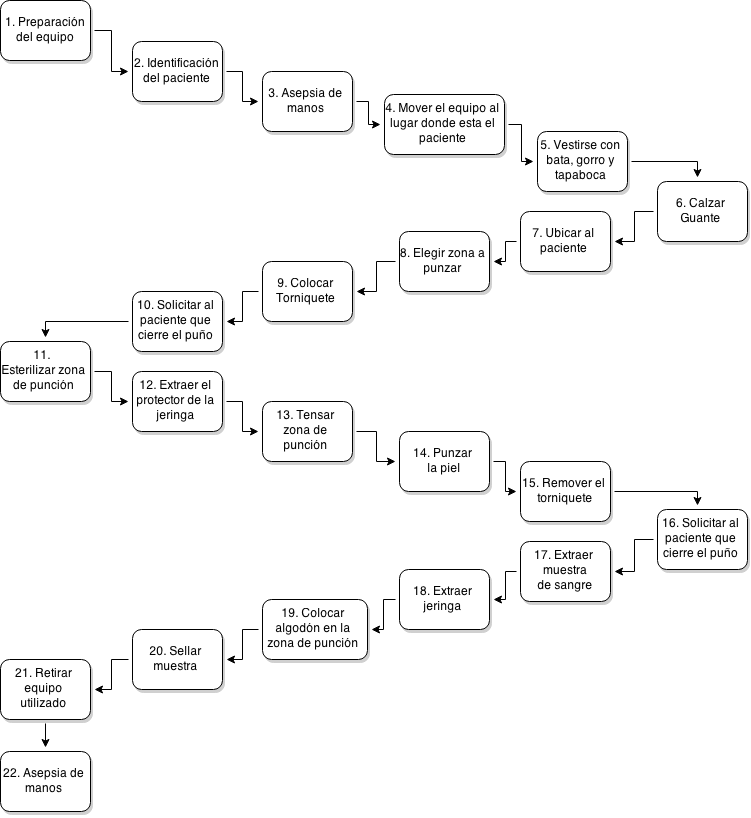
\includegraphics[scale=0.5]{requerimientos/images/hemocultivo.png}
\caption{Procedimiento de extracción de sangre.}
\label{fig:proc_hemocultivo}
\observacion{Se explica en algún lugar que no es necesariamente lineal? Por que
    se simplifica acá?}
\end{figure}

\begin{enumerate}
\item Preparar el equipo, lo que incluye seleccionar la jeringa adecuada.
\item Identificar al paciente, presentarse y explicarle el procedimiento que va
    a ser realizado.
\item Asepsia de las manos.
\item Llevar el equipo a la unidad en donde se encuentra el paciente.
\item Vestirse con bata estéril, tapaboca y gorro.
\item Calzarse los guantes.
\item Ubicar al paciente en posición adecuada, esto es, el brazo debe estar
    extendido y lo mas relajado posible.
\item Elegir la zona a puncionar, para ello se debe palpar la vena para
    averiguar sus características.
\item Colocar el torniquete, 6 a 10 centímetros por encima de la zona de
    punción.
\item Solicitar al paciente que cierre el puño.
\item Esterilizar la zona de punción.
\item Extraer el protector de la aguja.
\item Tensar la zona de punción.
\item Puncionar la piel con la aguja hacia arriba. La aguja se introduce con un
    ángulo de $10$ a $20$ grados.
\item Remover el torniquete.
\item Solicitar la apertura del puño.
\item Extraer la muestra de sangre necesaria.
\item Presionar y extraer la aguja.
\item Colocar algodón con alcohol en el punto de punción.
\item Sellar la muestra y enviarlo a su destinatario.
\item Retirar el equipo utilizado, incluyendo bata, tapaboca, gorro y guantes.
\item Asepsia de las manos.
\end{enumerate}


\subsection{Valoración de la escala de Glasgow}
\label{sec:glasgow}

La escala de Glasgow es utilizada como una herramienta de valoración objetiva
del estado de conciencia de pacientes en estado crítico\cite{protocolo}. La
escala consiste en la evaluación de tres criterios de observación clínica,
los cuales son: 
\begin{enumerate*}[label=\itshape\alph*\upshape.]
\item la respuesta ocular
\item la respuesta verbal, y
\item la respuesta motora.
\end{enumerate*}

\begin{table}[!hbt]
\centering
\begin{tabular}{llr}
\toprule
\textbf{Severidad} & 
\textbf{Puntuación} \\ 
\midrule
 Leve & 13 a 15 \\
 Moderado & 9 a 12 \\
 Grave & 3 a 8 \\
\bottomrule
\end{tabular}
\caption{Escala de valoración del estado del paciente\cite{helmick2007mild}.}
\label{tab:seleccion_glasgow_estado}
\end{table}

El puntaje que determina el estado del paciente se obtiene sumando la valoración
de cada una de las respuestas, en la figura~\ref{tab:seleccion_glasgow_estado}
se observan los posibles diagnósticos. A la vez cada respuesta se evalúa
mediante una escala independiente una de otra, donde cada respuesta se puntúa
con un número\cite{glasgow:doc}, los valores de cada respuesta se observan en las
tablas~\ref{tab:seleccion_glasgow_respuestas_ocular},~\ref{tab:seleccion_glasgow_respuestas_motor}
y~\ref{tab:seleccion_glasgow_respuestas_verbal}.

\begin{table}[!hbt]
\centering
\begin{tabular}{lr}
\toprule
\textbf{Apertura ocular} & \textbf{Valor} \\
\midrule
Espontánea & 4 \\
Al hablar & 3 \\
Al dolor & 2 \\
Ausente & 1 \\
\bottomrule
\end{tabular}
\caption{Valoración de las distintas respuestas en la escala de Glasgow,
    respecto a la reacción ocular}
\label{tab:seleccion_glasgow_respuestas_ocular}
\end{table}

\begin{table}[!hbt]
\centering
\begin{tabular}{lr}
\toprule
\textbf{Respuesta motora} & \textbf{Valor} \\
\midrule
Obedece & 6 \\
Localiza & 5 \\
Retira & 4 \\
Flexión anormal & 3 \\
Extiende & 2 \\
Ausente & 1 \\
\bottomrule
\end{tabular}
\caption{Valoración de las distintas respuestas en la escala de Glasgow,
    referentes a las respuestas motoras}
\label{tab:seleccion_glasgow_respuestas_motor}
\end{table}

\begin{table}[!hbt]
\centering
\begin{tabular}{lr}
\toprule
\textbf{Respuesta verbal} & \textbf{Valor} \\
\midrule
Orientada & 5 \\
Confusa & 4 \\
Palabras inapropiadas & 3 \\
Palabras incomprensibles & 2 \\
Ausente & 1 \\
\bottomrule
\end{tabular}
\caption{Valoración de las distintas respuestas en la escala de Glasgow
    referentes a la respuesta verbal}
\label{tab:seleccion_glasgow_respuestas_verbal}
\end{table}

El procedimiento se utiliza cuando existe un paciente con un estado de
conciencia indefinido, normalmente después de un accidente donde el paciente
recibió un traumatismo severo. El profesional que se encarga de evaluar debe
verificar el estado del paciente mediante
\begin{enumerate*}[label=\itshape\alph*\upshape.]
\item preguntas sencillas,
\item estímulos, e
\item inspecciones de partes del cuerpo.
\end{enumerate*}. 
Una vez que se obtiene una valoración individual para los aspectos
motor, ocular y visual del paciente, se obtiene la suma de las valoraciones y se
obtiene un puntaje para el estado del paciente.

El procedimiento de diagnóstico utilizando la escala de Glasgow es considerado
como uno de los apropiados para la solución propuesta ya que:

% Recheckear esto
\begin{itemize}
\item Permite la exploración del entorno pues hay diferentes formas de evaluar cada
    estado del paciente.
\item Es rara vez utilizado, pues las condiciones necesarias para que un paciente 
    requiera que se le realice este procedimiento son críticas, son
    escasas las oportunidades presentadas a los estudiantes durante sus
    prácticas de campo. 
\item La cantidad de reacciones que evalúa el procedimiento es muy alta,
    así, es difícil que un alumno pueda evaluar todos los posibles estados en
    sus prácticas de campo.
\item No es un procedimiento complejo, pues no requiere la manipulación de
    elementos, aún así requiere pericia y debe ser realizado en el menor tiempo
    posible.
\end{itemize}


\subsubsection{Evaluación al alumno}

En este apartado se detallan las competencias básicas relacionadas al procedimiento de 
valoración de la escala de Glasgow según el plan de estudios de los
estudiantes de enfermería del \Gls{iab} y los criterios relacionados al procedimiento 
según la planilla de práctica que poseen los profesores instructores para evaluar al alumno.

La competencia básica que incluye a la evaluación del paciente mediante la
escala de Glasgow es:

\begin{itemize}
\item Identificar actividades de cuidados según problemas urgentes principales.
\end{itemize}

En el gráfico~\ref{fig:proc_glasgow} se observan los pasos necesarios para
realizar la evaluación utilizando la escala de Glasgow\cite{protocolo}. Dentro del
procedimiento definido en la práctica profesional los criterios son:

\begin{figure}
\centering
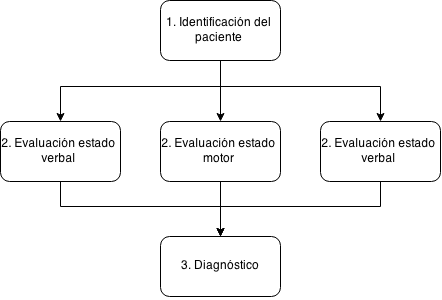
\includegraphics[scale=0.5]{requerimientos/images/glasgow.png}
\caption{Evaluación de Glasgow.}
\label{fig:proc_glasgow}
\end{figure}

\begin{itemize}
\item Control de signos vitales.
\item Inspección cefalocaudal, 
\item Evaluación utilizando escala de Glasgow.
\item Preparación del equipo según prioridad del problema
\item Analizar su participación en las actividades.
\item Fundamenta científicamente sus decisiones.
\end{itemize}

Se observa que el punto \enquote{Evaluación utilizando escala de Glasgow}, es un
paso necesario para la evaluación inicial de un paciente en estado crítico.

\subsubsection{Protocolo del procedimiento}
\label{sec:glasgow_protocolo}

Los pasos requeridos en el protocolo del procedimiento según~\cite{protocolo} y los 
profesores del \Gls{iab} son los siguientes:

\begin{enumerate}
\item Preparación del material
\item Preparación del paciente: comprobar su identidad, mantener una ambiente
    tranquilo evitando interrupciones, requerir la atención del paciente.
\item Colocar al paciente en posición cómoda.
\item Medir la apertura ocular.
\item Evaluar la respuesta motora.
\item Medir la respuesta verbal.
\item Registrar la puntuación final obtenida.
\end{enumerate}
